\documentclass{scrartcl}

\usepackage{graphicx}
\usepackage[utf8]{inputenc}
\usepackage[T1]{fontenc}
\usepackage{lmodern}
\usepackage{babel}
\usepackage{amsmath}
\usepackage{amsthm}
\usepackage{mathtools}
\usepackage{amssymb}
\usepackage{listings}
\usepackage{xparse}
\usepackage{geometry}
\usepackage{enumerate}
\usepackage{tikz}
\usepackage[style=english]{csquotes}
\usepackage[language=english, backend=biber, style=alphabetic, sorting=nyt]{biblatex}

\usetikzlibrary{babel, positioning, shapes.geometric, arrows, arrows.meta}
\addbibresource{bibliography.bib}

\title{SIKE - A key exchange scheme based on Supersingular Elliptic Curves}
\author{Simon Pohmann}

\newcommand{\N}{\mathbb{N}}
\newcommand{\Z}{\mathbb{Z}}
\newcommand{\F}{\mathbb{F}}
\newcommand{\proj}{\mathrm{proj}}
\newcommand{\Quot}{\mathrm{Quot}}
\renewcommand{\O}{O}

\newtheorem{prop}{Proposition}[section]
\newtheorem{theorem}[prop]{Theorem}
\newtheorem{corollary}[prop]{Corollary}
\newtheorem{alg}[prop]{Algorithm}
\newtheorem{definition}[prop]{Definition}
\newtheorem{example}[prop]{Example}
\newtheorem{remark}[prop]{Remark}

\begin{document}

\maketitle

\tableofcontents

\section{Elliptic Curves}

\subsection{Elliptic Curves as (projective) Varieties}

For this work, we define elliptic curves as certain varieties in the projective plane over $\bar{K}$ as follows.

\begin{definition}
    A (possibly nonsmooth) elliptic curve $E$ defined over a field $K$ is the (projective) zero set
    \begin{equation*}
        E = \mathcal{Z}_{\bar{K}}(Y^2Z + a_1 XYZ + a_3 YZ^2 - X^3 - a_2 X^2 Z - a_4 X Z^2 - a_6 Z^3) \subseteq \mathbb{P}_{\bar{K}}^2
    \end{equation*}
    of some irreducible polynomial $Y^2Z + a_1 XYZ + a_3 YZ^2 - X^3 - a_2 X^2 Z - a_4 X Z^2 - a_6 Z^3 \in K[X, Y, Z]$.
    The point $\O := (0 : 1 : 0) \in E$ is called the point at infinity of the elliptic curve.
\end{definition}

It is convention to define an Elliptic Curve by the dehomogenization
\footnote{For a homogeneous polynomial $f \in K[x, y, z]$ the dehomogenization is $f(x, y, 1)$, denoted by $f^{\mathrm{deh}}$.}  
of its defining polynomials, i.e. say that the curve $E$ is defined by the equation
\begin{equation*}
    E: \ Y^2 + a_1 XY + a_3 Y = X^3 + a_2 X^2 + a_4 X + a_6
\end{equation*}
By homogenizing the polynomial equation, one can retrieve the original homogeneous polynomial, so this representation defines the Elliptic Curve uniquely.

Readers that are not used to working with projective geometry may also think of an Elliptic Curve as the (affine) set of solutions of this equation, together with a dedicated point $\O$ ``at infinity''.
Using this point of view, we will also identify affine points $(x, y)$ with $(x : y : 1)$.

Usually, one only considers elliptic curves that are smooth. 
This is a property that can be defined for all varieties, but here we will only give a definition applicable only to elliptic curves.
This relies on the so-called discriminant of an elliptic curve.

\begin{definition}
    \label{def:discriminant}
    A (possibly nonsmooth) elliptic curve $E$ defined by $Y^2 + a_1 XY + a_3 Y = X^3 + a_2 X^2 + a_4 X + a_6$ is called smooth, if the discriminant
    \begin{align*}
        \Delta(E) = & - b_2^2 b_8 - 8 b_4^3 - 27 b_6^2 + 9 b_2 b_4 b_6 \\
        \text{where} \ & b_2 = a_1^2 + 4 a_2 \\
        & b_4 = a_1 a_3 + 2 a_4 \\
        & b_6 = a_3^2 + 4 a_6 \\
        & b_8 = a_1^2 a_6 + 4 a_2 a_6 - a_1 a_3 a_4 + a_2 a_3^2 - a_4
    \end{align*}
    is nonzero. In this work, the term ``elliptic curve'' will be used for smooth elliptic curves.
\end{definition}

One can now check by a lengthy computation that having a nonzero discriminant is equivalent to having a well-defined tangent line at every point.
For the sake of brevity, we will only perform this computation for a simpler case later.

\subsection*{Isogenies}

In this section, we will introduce the notion of an isogeny, which are the structure-preserving maps between Elliptic Curves.
A crucial part of this definition are morphisms, which are the structure-preserving maps in the category of algebraic varieties.
Their theory is quite wide, and anything further than giving the definitions and some basic facts is beyond the scope of this work.
The interested reader is advised to refer to a book on Algebraic Geometry.
However, we try to give sufficient intuition that one can follow the rest of this work without a background in Algebraic Geometry.

\begin{definition}
    \label{def:rational_map}
    Given irreducible varieties $V = \mathcal{Z}_{\bar{K}}(I), W \subseteq \mathbb{P}_{\bar{K}}^2$, a partial map $\phi: V \to W$ is called rational if it is given locally by rational functions.
    Namely, $\phi$ is rational if there are homogeneous $f_1, f_2, f_3 \in \bar{K}[X, Y, Z]$ of same degree and not all zero such that for each point $(x : y : z) \in V$ at which $\phi$ is defined, there are ``equivalent'' homogeneous polynomials $(g_1, g_2, g_3) \in \bar{K}[X, Y, Z], \ (g_1, g_2, g_3) \sim (f_1, f_2, f_3)$ of same degree such that
    \begin{align*}
        (g_1(a), g_2(a), g_3(a)) &\neq (0, 0, 0) \quad \text{and}\\
        (g_1(a) : g_2(a) : g_3(a)) &= \phi((a_1 : a_2 : a_0))
    \end{align*}
    where $a = (x, y, z)$.

    Here we define equivalence as $(f_1, f_2, f_3) \sim (g_1, g_2, g_3)$ if $f_i g_j = f_j g_i \mod I$ for all $i, j$.
    We use the notation $\phi = [f_1^{\mathrm{deh}} / f_3^{\mathrm{deh}}, f_2^{\mathrm{deh}} / f_3^{\mathrm{deh}}, 1]$
    \footnote{Note that $f$ corresponds to $f^{\mathrm{deh}}$ uniquely except for scaling by $z$, but scaling by $z$ does not change the defined rational map. This ``affine'' notation corresponds to the use of dehomogenized polynomials for defining Elliptic Curves.}.
    The rational map is said to be defined over $K$, if $f_1, f_2, f_3 \in K[X, Y, Z]$.
\end{definition}

This definition is quite technical, as it is local in nature.
The intuition is that each coordinate of such a map is given by a quotient of polynomials
(or, as projective points are invariant under scaling of their coefficients, just by polynomials).
However, this means we cannot define a correct value for the map if evaluating the polynomials yields ``$\frac 0 0$'' or ``$(0 : 0 : 0)$''.
Now one can define such a polynomial function on a somewhat bigger set by using a local definition as explained above:
We use different ``representations'' by polynomials for different subsets of the domain on which they are defined, and require that two of them coincide on points at which both are defined.
For more information, the reader should refer to a book on Algebraic Geometry.

Note that we still defined rational maps as partial maps, i.e. although we use a local definition, it is possible that no value is defined for a certain point.
Rational maps that are not partial are then the ``nice'' maps of Algebraic Geometry.

\begin{definition}
    A rational map between varieties that is defined everywhere is called morphism. If it is bijective and its inverse is a morphism, it is called a variety isomorphism.
\end{definition}

As we will see in the next part, Elliptic Curves contain more structure than just the geometric one.
Thus we will work with the stronger notion than that of a morphism.

\begin{definition}
    A morphism $\phi$ between Elliptic Curves $E_1, E_2$ is called isogeny, if $\phi(\O) = \O$.
    A bijective isogeny whose inverse is also an isogeny is called isomorphism.
\end{definition}

Similar to the convention of defining Elliptic Curves by dehomogenized polynomials, we will use a notation that does not rely on homogeneous coordinates.
For this, we require the coordinate ring of an Elliptic Curve, which is the ring of ``polynomial functions'' defined on the curve.

\begin{definition}
    Let $E$ be an Elliptic Curve defined by the polynomial $F(X, Y) = Y^2 + a_1 XY + a_3 Y - X^3 - a_2 X^2 - a_4 X - a_6$.
    Then the ring $K[E] := K[X, Y] / (F(X, Y))$ is called the (affine) coordinate ring of $E$.
    Its field of fractions is called the function field of $E$ and denoted by $K(E)$.
\end{definition}

\begin{prop}
    Let $E_1, E_2$ be Elliptic Curves and $\phi: E_1 \to E_2$ be a map with $\phi(\O) = \O$.
    Then the following are equivalent:
    \begin{itemize}
        \item $\phi$ is an isogeny
        \item There are elements $u, v \in K(E)$ such that for all $a = (x, y) \in E$ there are polynomials $g_1, g_2, g_3 \in K[X, Y]$ with
        \begin{equation*}
            \frac {\overline{g_1}} {\overline{g_3}} = u, \ \frac {\overline{g_2}} {\overline{g_3}} = v \quad \text{in $K(E)$}
        \end{equation*}
        and
        \begin{equation*}
            g_3(a) \neq 0, \ \phi(a) = \Bigl( \frac {g_1(a)} {g_3(a)}, \frac {g_2(a)} {g_3(a)} \Bigr) \quad \text{or} \quad (g_1(a), g_2(a)) \neq (0, 0), \ \phi(a) = \O
        \end{equation*}
    \end{itemize}
    In this case we use the notation $\phi = [u, v, 1]$.
\end{prop}
\begin{proof}
    For $\Leftarrow$ we have to show that $\phi$ is an isogeny, i.e. show the condition from \ref{def:rational_map}.
    Let $f_1, f_2, f_3 \in K[X, Y, Z]$ homogeneous of same degree such that $f_1^{\mathrm{deh}} / f_3^{\mathrm{deh}}$ is a representative of $u$ and $f_2^{\mathrm{deh}} / f_3^{\mathrm{deh}}$ is a representative of $v$.
    For a point $(x : y : z) \neq \O$ we have wlog that $z = 1$, so $(x : y : z) = (x, y)$.
    
    Let now be $g_1, g_2, g_3 \in K[X, Y]$ the polynomials given by the assumption and $d = \max \{ \deg g_1, \deg g_2, \deg g_3 \}$.
    Then the polynomials $g_i' := g_i^{\mathrm{hom}} Z^{d - \deg g_i}$ are equivalent to $f_1, f_2, f_3$ as in \ref{def:rational_map}.
    If $g_3(a) \neq 0$ have
    \begin{equation*}
        \phi(a) = \Bigl( \frac {g_1(a)} {g_3(a)}, \frac {g_2(a)} {g_3(a)} \Bigr) = ( g_1(a) : g_2(a) : g_3(a) )
    \end{equation*} 
    and clearly $(g_1(a), g_2(a), g_3(a)) \neq (0, 0, 0)$.

    Otherwise have $\phi(a) = \O$ and $g_3 = 0, \ (g_1(a), g_2(a)) \neq (0, 0)$.
    Thus clearly\\$(g_1(a), g_2(a), g_3(a)) \neq (0, 0, 0)$ and $p := (g_1(a) : g_2(a) : g_3(a)) = (g_1(a) : g_2(a) : 0)$ is a point on the hyperplane at infinity $H = \mathcal{Z}_{\bar{K}}(Z)$.
    As $H \cap E = \{ \O \}$ get $p = \O$ and thus $\phi(a) = \O = (g_1(a) : g_2(a) : g_3(a))$.

    The direction $\Rightarrow$ works similarly, but instead of homogenizing the polynomials from the assumption we dehomogenize them, i.e. we choose
    \begin{equation*}
        u = \frac {\overline{f_1^{\mathrm{deh}}}} {\overline{f_3^{\mathrm{deh}}}}, \ v = \frac {\overline{f_2^{\mathrm{deh}}}} {\overline{f_3^{\mathrm{deh}}}} \quad \text{and} \quad g_i' = g_i^{\mathrm{deh}}
    \end{equation*}
\end{proof}

\begin{prop}
    Let $E_1, E_2$ be Elliptic Curves such that $E_2$ is defined by the equation $F(X, Y) = 0$ for $F \in \bar{K}[X, Y]$ and let $u, v \in \bar{K}(E_1)$ with $F(u, v) = 0 \in \bar{K}(E_1)$.
    Then there is a unique isogeny $\phi: E_1 \to E_2$ such that $\phi = [u, v, 1]$.
\end{prop}
\begin{proof}
    The uniqueness is clear, as each representative of $u$ resp. $v$ yields the same value when evaluated at a point on the curve.
    To show the existence, it suffices to show that for each $a = (a_1, a_2) \in E_1$ there are polynomials $g_1, g_2, g_3 \in K[X, Y]$ such that $g_1/g_3$ and $g_2/g_3$ are representatives of $u$ resp. $v$ and $(g_1(a), g_2(a), g_3(a)) \neq (0, 0, 0)$.
    These polynomials $g_1, g_2, g_3$ then give a well-defined value for $\phi(a)$.

    As $E_1$ is smooth, we get that the localization $K[E_1]_a$ of $K[E_1]$ at the maximal ideal $(X - a_1, Y - a_2)$ is a discrete valuation domain (\cite[II.1.1]{arithmetic_elliptic_curves}).
    Hence, $K[E_1]_a$ has a uniformizer $t \in K[E_1]$. 
    Now let $u = u_1 / u_2$ and $v = v_1 / v_2$ for $u_1, u_2, v_1, v_2 \in K[E_1]$.
    Then claim the follows with
    \begin{equation*}
        g_1 = t^{-d} u_1v_2, \quad g_2 = t^{-d} v_1u_2, \quad g_3 = t^{-d} v_2u_2
    \end{equation*}
    where
    \begin{equation*}
        d = \min \{ \mathrm{val}_t(u_1v_2), \mathrm{val}_t(v_1u_2), \mathrm{val}_t(v_2u_2) \} \in \N
    \end{equation*}
    and $\mathrm{val}_t$ is the valuation is the DVD $K[E_1]_a$.
\end{proof}

\subsection{A simpler formula}

The general Weierstraß equation is still relatively complicated. If the characteristic of $K$ is not $2$ or $3$ however, we have the following simpler representation:

\begin{prop}
    Let $E$ be an elliptic curve defined over $K$ with $\mathrm{char}(K) \neq 2, 3$ by the Weierstraß equation $y^2 + a_1 xy + a_3 y = x^3 + a_2 x^2 + a_4 x + a_6$.
    Then $E$ is isomorphic to an elliptic curve defined by a Weierstraß equation of the form
    \begin{equation*}
        y^2 = x^3 + Ax + B
    \end{equation*}
    where $A, B \in K$.
\end{prop}
\begin{proof}
    Consider the isogeny given by
    \begin{equation*}
        \phi_1 = \Bigl[ x, y - \frac {a_1 x + a_3} 2, 1 \Bigr]
    \end{equation*}
    Then have that
    \begin{align*}
        &\left( y - \frac {a_1 x + a_3} 2 \right)^2 + (a_1 x + a_3) \left( y - \frac {a_1 x + a_3} 2 \right) \\
        = & \ y^2 - y (a_1 x + a_3) + (a_1 x + a_3) y - \left( \frac {a_1 x + a_3} 2 \right)^2 = y^2 - \frac 1 4 ( a_1 x + a_3 )^2
    \end{align*}
    Let $E_1$ be the elliptic curve defined by 
    \begin{equation*}
        E_1: y^2 = x^3 + \frac 1 4 b_2 x^2 + \frac 1 2 b_4 x + \frac 1 4 b_6
    \end{equation*}
    with $b_2 = 4a_2 + a_1^2$, $b_4 = 2 a_4 + a_1 a_3$ and $b_6 = 4a_6 + a_3^2$.
    Then $\phi_1$ maps $E_1$ to $E$ as by the above computation, $\phi(x : y : z) \in E$ for all $(x : y : z) \in E_1$.
    Furthermore, $\phi_1$ is given by a linear change of coordinates, hence it is an isomorphism.

    Similarly, consider the isogeny given by
    \begin{equation*}
        \phi_2 = \Bigl[ x - \frac {b_2} {12}, y, 1 \Bigr]
    \end{equation*}
    By an analogous computation as above, get that $\phi_2$ is an isomorphism $E_2 \to E_1$ where $E_2: y^2 = x^3 + Ax + B$ for $A = \frac 1 2 (b_4 - \frac 1 {24} b_2^2)$ and $B = \frac 1 4 (\frac 1 6 b_2 b_4 - \frac 1 {216} b_2^3 - b_6)$.
    Composing $\phi_1 \circ \phi_2$ yields an isomorphism between $E_2$ and $E$.
\end{proof}

The reader might compare the $b_2, b_4, b_6$ used in this proof with the definition of the discriminant \ref{def:discriminant} to get an explanation for the choice of some parts of the discriminant formula.
This formula also gets much simpler when using the simplified form.

\begin{remark}
    Let $E$ be an elliptic curve defined by $E: y^2 = x^3 + Ax + B$. Then
    \begin{equation*}
        \Delta(E) = -16(27 B^2 + 4 A^3)
    \end{equation*}
\end{remark}
\begin{proof}
    Just insert $a_4 = A, a_6 = B$ and $a_1 = a_2 = a_3 = 0$ into the definition \ref{def:discriminant}.
\end{proof}

For simplicity, we will from now on assume that the characteristic of $K$ is not $2$ or $3$ and hence use this simpler formula. 
Most proofs work also in the general case, but the involved computations will be more complicated and less instructive.

\subsection{More isomorphisms}

Until now we have seen that each curve is isomorphic to a curve given by a relatively simple equation.
To completely classify whether two curves are isomorphic, it is now left to study when two curves of this form are isomorphic.
This can be done by the so-called j-invariant.

\begin{definition}
    Let $E$ be an elliptic curve defined by $E: y^2 = x^3 + Ax + B$. Then the j-invariant is given by
    \begin{equation*}
        j(E) := \frac {(-48 A)^3} {\Delta(E)} = 1728 \frac {4A^3} {27 B^2 + 4A^3}
    \end{equation*}
\end{definition}

\begin{prop}
    \label{prop:j_invariant}
    Let $E: y^2 = x^3 = Ax - B$ and $E': y^2 = x^3 - A'x - B'$ be elliptic curves. Then there is an isomorphism $E \to E'$ if and only if $j(E) = j(E')$.
\end{prop}
\begin{proof}
    First, assume $j(E) = j(E')$ and consider the isogeny $\phi = [u^2 x, u^3 y, 1]$ where $u^4 = A/A'$.
    Then
    \begin{align*}
        (u^3 y)^2 =& \ u^6 y^2 \quad \text{and} \\
        (u^2 x)^3 - A (u^2 x) - B =& \ u^6 \Bigl(x^3 - \frac 1 {u^4} A x - \frac 1 {u^6} B \Bigr) \\
        =& \ u^6 \Bigl( x^3 - A' x - \frac 1 {u^6} B \Bigr)
    \end{align*}
    From $j(E) = j(E')$ we get
    \begin{equation*}
        A^3 (27 B'^2 + 4A'^3) = A'^3 (27 B^2 + 4A^3)
    \end{equation*}
    Thus
    \begin{equation*}
        A^3 \left( 27 B'^2 + 4\frac 1 {u^{12}} A^3 \right) = \frac 1 {u^{12}} A^3 (27 B^2 + 4A^3)
    \end{equation*}
    and so
    \begin{equation*}
        B'^2 = \frac 1 {u^{12}} B^2 + \frac 1 {27 u^{12}} (4 A^3 - 4 A^3) = \frac 1 {u^{12}} B^2
    \end{equation*}
    It follows that $u^6 = B/B'$ and so $\phi$ maps $E$ to $E'$. It is only a linear transformation, hence also an isomorphism.

    For the other direction, assume there is an isomorphism $\phi = [x', y', 1]$ from $E$ to $E'$ where $E': y^2 = x^3 + A'x + B'$ and $x', y' \in K[E]$.
    \paragraph{Claim} Then $x = u_1 x' + r$ and $y = u_2 y' + x_2 x' + t$ for $u_1, u_2 \in \bar{K}^*$ and $r, t \in \bar{K}$.
    To prove this claim, we require some advanced Algebraic Geometry. 
    To examine $\O$ using an ``affine'' approach, we change our embedding $K^2 \to \mathbb{P}^2$ such that $(x, z) \mapsto (x : 1 : z)$ and get the affine curve
    \begin{align*}
        E \ &\text{defined by} \ Z = X^3 + A X Z^2 + B Z^3 \ \text{resp.} \\
        E' \ &\text{defined by} \ Z = X^3 + A' X Z^2 + B' Z^3
    \end{align*}
    The curves do not change by this, we just consider another affine part of the projective plane that now contains $\O$. In particular, $\O$ is now the origin $(0, 0)$.
    Note that this is just a conceptual tool, formally this is given by the isomorphism 
    \begin{align*}
        K(E) &= \Quot\left(K[x, y] / (y^2 - x^3 - A x - B)\right) \\
        \cong \ K(\tilde{E}) &= \Quot\left(K[X, Z]/(Z - X^3 - A X Z^2 - B Z^3)\right)
    \end{align*}
    via $x \mapsto X/Z, \ y \mapsto 1/Z$, where $\tilde{E} = E \cap K^2$ is the considered affine part of the curve. 
    We identify those two representations, in particular have $x, y, x', y' \in K(\tilde{E})$.
    
    Now consider the localization
    \begin{equation*}
        R := K[\tilde{E}]_{(0, 0)} := K[\tilde{E}]_{\mathfrak{m}} \subseteq K(\tilde{E}) \ \text{where} \ \mathfrak{m} = \langle x, z \rangle = \{ f \in K[\tilde{E}] \ | \ f(0, 0) = 0 \}
    \end{equation*}
    of the affine coordinate ring $K[\tilde{E}] = K[X, Z]/(Z - X^3 - A X Z^2 - B Z^3)$ at $(0, 0) \in K^2$.
    This is a local ring with unique maximal ideal $\mathfrak{m}$.
    We show that the valuation of $X$ and $X' := x'/y'$ in $R$ is -2.
    Now have that $Z = X^3 + A X Z^2 + B Z^3$ and hence
    \begin{equation*}
        \underbrace{\left( 1 - B Z^2 \right)}_{=:\ \alpha \ \in R^*} Z = X (Z^2 + A Z^2)
    \end{equation*}
    It follows that $Z \in \langle X \rangle$ and thus $\mathfrak{m} = \langle X \rangle$.
    Furthermore have $X (X^2 + A Z^2) = X (X^2 + A \alpha X^2) = X^3 (1 + A \alpha)$ and $1 + A \alpha$ is a unit.
    Therefore $\langle X \rangle^3 = \langle Z \rangle$ and thus $x = X / Z$ has valuation $1 - 3 = -2$.
    The same calculation for $X' := x' Z', Z' := 1/y'$ shows that $x' = X' / Z'$ has valuation -2.
    Here we require that $\phi$ maps $\O$ to $\O$, as then $Z' \in \mathfrak{m}$ and hence $\alpha' = 1 - B' Z'^2$ is a unit.
    The Riemann-Roche theorem tells us that
    \begin{equation*}
        V_2 := \{ f \in K(E)^* = K(\tilde{E})^* \ | \ \text{valuation of $f$ in $R$} \geq -2 \} \cup \{ 0 \}
    \end{equation*}
    is a 2-dimensional $K$-vector space. By the above, $x, x' \in V_2$ and thus there must be a linear dependency between $1, x$ and $x'$.
    By an analogue computation we also find a linear dependency between $1, x, y, y'$ as the corresponding $V_3$ is 3-dimensional by Riemann-Roche.
    This shows the claim.

    Now we have $x'^3 + A' x' + B' = y'^2$ and by plugging in the linear transformation $x' = (x - r) / u_1$ and $y' = (y - t - s_2 x') / u_2$ one can compute that $j(E) = j(E')$.
\end{proof}

\section{The group structure}

Apart from the geometric nature of an elliptic curve, they have additional important structure: Elliptic curves are groups.
In particular for cryptography, this is crucial. 
In this section, we will see how this group structure looks like.

\begin{prop}
    \label{prop:bezout_theorem_case}
    Let $E$ be an elliptic curve. Then each projective line meets $E$ at exactly three points, with multiplicity.
\end{prop}

\begin{definition}
    Define a map
    \begin{equation*}
        +_{\mathrm{geo}}: E \times E \to E
    \end{equation*}
    that for $P, Q \in E$ is given by the following geometric construction:
    \begin{itemize}
        \item Let $L$ be the line through $P, Q$ (with multiplicity)
        \item Let $R$ be the third point of intersection of $E$ with $L$ (exists by \ref{prop:bezout_theorem_case})
        \item Let $L'$ be the line through $R, \O$
        \item Set $P +_{\mathrm{geo}} Q$ to be the third point of intersection of $E$ with $L'$
    \end{itemize}
\end{definition}

Two special cases can occur in this construction: If $P = Q$ or $R = \O$ then the ``with multiplicity'' is important, so the line $L$ resp. $L'$ is chosen to be the tangent at that point.
Furthermore, if we construct a line through $\O$ and a second point $P$, this has the following, affine interpretation: It is the unique line containing $P$ that is parallel to the y-axis.
Combining these two, we see that the unique line through $\O$ and $\O$ must be the line at infinity (which only exists in the projective space), whose third point of intersection with $E$ is again $\O$.
So have the following special cases
\begin{align*}
    &P +_{\mathrm{geo}} \O = \O +_{\mathrm{geo}} P = P \\
    &(x, y) +_{\mathrm{geo}} (x, -y) = (x, -y) +_{\mathrm{geo}} (x, y) = \O
\end{align*}

Now we consider a second binary operation $+_{\mathrm{alg}}$ on $E$. This will be described using algebra, hence we require the following theorem.

\begin{prop}
    \label{prop:dedekind_domain}
    Let $E: y^2 = x^3 + Ax + B$ be an elliptic curve. Then the affine coordinate ring $\bar{K}[E]$ is a Dedekind domain and there is a bijection
    \begin{equation*}
        \phi: E \to \mathrm{Cl}(\bar{K}[E]), \quad (\lambda, \mu) \mapsto \overline{\langle x - \lambda, y - \mu \rangle}, \ \O \mapsto \overline{\langle 1 \rangle}
    \end{equation*}
\end{prop}
\begin{proof}
    See the (unpublished) lecture notes \cite{lecture_notes_crypta}.
\end{proof}

\begin{definition}
    Define the map
    \begin{equation*}
        +_{\mathrm{alg}}: E \times E \to E, \quad (P, Q) \mapsto  \phi^{-1}(\phi(P) \phi(Q))
    \end{equation*}
\end{definition}

Lastly, we look at a third operation $+_{poly}$ that is given explicitly by rational functions.

\begin{definition}
    Define the map 
    \begin{align*}
        +_{\mathrm{poly}}: E \times E \to E, \quad ((x_1, y_1), (x_2, y_2)) &\mapsto (x_3, y_3), \\
        (\O, P), (P, \O) &\mapsto P \\
        ((x, y), (x, -y)) &\mapsto \O
    \end{align*}
    where for $P = (x_1, y_1), \ Q = (x_2, y_2) \neq (x_1, -y_1)$ we set
    \begin{align*}
        \lambda &:= \begin{cases}
            \frac {y_2 - y_1} {x_2 - x_1} \ \text{if} \ x_1 \neq x_2 \\
            \frac {3 x_1^2 + A} {2 y_1} \ \text{otherwise}
        \end{cases} \\
        x_3 &:= -x_1 - x_2 + \lambda^2 \\
        y_3 &:= -y_1 + \lambda (x_1 - x_3)
    \end{align*}
\end{definition}

Note that $+_{\mathrm{poly}}$ is given by polynomials. We do not consider the general case here, but note that both the ``translation'' map and the ``scalar multiplication'' map are morphisms:
Let $P = (u, v) \in E$ and consider the map $\tau_P: E \to E, \ Q \mapsto Q + P$.
In $K(E)$ we have
\begin{equation*}
    \frac {v - y} {u - x} = \frac {v^2 - y^2} {(u - x)(v + y)} = \frac {u^3 + Au - x^3 - Ax} {(u - x)(v + y)} = \frac {u^2 + ux + x^2 + A} {v + y}
\end{equation*}
and so 
\begin{equation*}
    \tau_P = [-u - x + \lambda^2, \ -y_1 + \lambda (x - \lambda^2), 1] \ \text{where} \ \lambda = \frac {v - y} {u - x} \in K(E)
\end{equation*}
is a morphism ($\lambda$ is regular everywhere except at $(u, -v)$, but here we clearly get $\O$).

Similarly, the scalar multiplication 
\begin{equation*}
    [m]: E \to E, \ Q \mapsto \underbrace{Q + ... + Q}_{m \ \text{times}}
\end{equation*}
is a morphism and hence an isogeny (almost the same calculation).

Now we get the fundamental result on the group structure of elliptic curves.

\begin{prop}
    \label{prop:group_operation}
    Let $E: y^2 = x^3 + Ax + B$ be an elliptic curve. Then $+ := +_{\mathrm{geo}} = +_{\mathrm{alg}} = +_{\mathrm{poly}}$.
\end{prop}

Now combining the well-known properties of the different definitions of $+$, we get the

\begin{corollary}
    Let $E: y^2 = x^3 + Ax + B$ be an elliptic curve. Then 
    \begin{itemize}
        \item $E$ together with the binary operation $+$ from \ref{prop:group_operation} is a group.
        \item $E$ has neutral element $\O$
        \item $E$ is abelian
        \item the $K$-rational points $E(K) := E \cap \mathbb{P}_K^2$ form a subgroup
    \end{itemize}
\end{corollary}

This now gives rise to a group structure.

\begin{definition}
    Let $E: y^2 = x^3 + Ax + B$ be an elliptic curve. Then we endow $E$ with a group structure, where $\O$ is the neutral element and the map from \ref{prop:group_operation} is the group operation.
\end{definition}

\section{Isogenies}

In \ref{def:isogeny} we have already defined what an isogeny is.
Since this work is about isogeny-based cryptography, they will play a crucial role in the following parts.
Hence it is important that we study the properties of isogenies in more detail.

A very fascinating and fundamental result is that isogenies are group homomorphisms.
\begin{prop}
    \label{prop:isogeny_homomorphism}
    Let $E, E'$ be elliptic curves and $\psi: E \to E'$ an isogeny. Then $\psi$ is a group homomorphisms.
\end{prop}
\begin{proof}
    Have $\psi = [\psi_1, \psi_2, \psi_3]$ with $\psi_i \in K[E]$ and consider the ring homomorphism
    \begin{equation*}
        \psi^*: \bar{K}[E'] \to \bar{K}[E], \quad \overline{f} \mapsto \overline{f^{\mathrm{hom}}\left(\psi_1, \psi_2, \psi_3\right)}
    \end{equation*}
    This is well-defined, as if $\overline{f} = \overline{g} \in \bar{K}[E']$, then $f - g$ vanishes on $E'$ an thus $f(\psi_1, \psi_2, \psi_3) - g(\psi_1, \psi_2, \psi_3)$ vanishes everywhere, thus is zero.
    Note that
    \begin{equation*}
        f^{\mathrm{hom}}(\psi_1, \psi_2, \psi_3) = \psi_3^d \ f\left(\frac {\psi_1} {\psi_3}, \frac {\psi_2} {\psi_3}\right) \ \text{for some} \ d \in \N
    \end{equation*}
    and in the class group $\mathrm{Cl}(\bar{K}[E])$ have further $\overline{\langle \psi_3 \rangle} = 1$.
    Now we have by \ref{prop:dedekind_domain} that the following diagram is commutative
    
    \begin{center}
    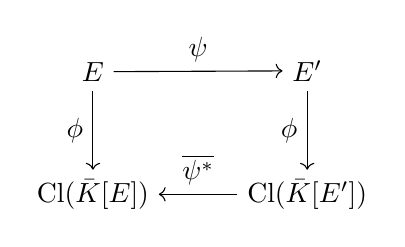
\begin{tikzpicture}
        \node (E) {$E$};
        \node[below = of E] (KE) {$\mathrm{Cl}(\bar{K}[E])$};
        \node[right = of KE] (KEp) {$\mathrm{Cl}(\bar{K}[E'])$};
        \node[above = of KEp] (Ep) {$E'$};

        \draw[->] (E) -- (Ep) node[midway, above] {$\psi$};
        \draw[->] (E) -- (KE) node[midway, left] {$\phi$};
        \draw[->] (Ep) -- (KEp) node[midway, left] {$\phi$};
        \draw[->] (KEp) -- (KE) node[midway, above] {$\overline{\psi^*}$};
    \end{tikzpicture}
    \end{center}
    Clearly $\overline{\psi^*}: \mathrm{Cl}(\bar{K}[E']) \to \mathrm{Cl}(\bar{K}[E])$ is a group homomorphism, and by \ref{prop:group_operation} we know that $\phi$ is a group isomorphism.
    The claim follows.
\end{proof}

\begin{prop}
    Let $E, E'$ be elliptic curves and $\psi: E \to E'$ a nonconstant isogeny. Then $\ker\psi \subseteq E$ is finite.
\end{prop}
\begin{proof}
    The fiber
    \begin{equation*}
        V := \ker\psi = \psi^{-1}(\{ \O \})
    \end{equation*}
    is a variety (it is the intersection of $Z(\langle \psi_1, \psi_3, \psi_2 - 1 \rangle) \cup Z(\langle \psi_1, \psi_2, \psi_3 \rangle)$, where $(\psi_1, \psi_2, \psi_3)$ runs through all representations of $\psi$, because for each preimage point, there is a representation such that the point is not in $Z(\langle \psi_1, \psi_2, \psi_3\rangle)$).

    We have $E \not\subseteq V$ as $\psi$ is nonconstant. So $E$ is a proper subvariety of $E$, an as $E$ is irreducible, it follows that $V$ is 0-dimensional, hence finite.
\end{proof}

The map $\psi^*$ considered in \ref{prop:isogeny_homomorphism} is indeed quite important, as it induces a field extension
\begin{equation*}
    \bar{K}(E) \ | \ \psi^*(\bar{K}(E'))
\end{equation*}
Using this, we can describe certain properties of isogenies.

\begin{definition}
    An isogeny $\psi: E \to E'$ is called separable, if the corresponding field extension $\bar{K}(E) | \psi^*\bar{K}(E)$ is separable.
\end{definition}

There are many nice propositions in this context. For example, the field extension $\bar{K}(E) | \psi^*\bar{K}(E)$ is always finite, and if the isogeny is separable, then its degree is equal to $\#\ker\psi$.
This is not fundamental for the cryptosystem we consider later, but keeping it in mind helps with understanding the following theorems.

\begin{prop}
    \label{prop:unique_isogeny}
    Let $E$ be an elliptic curve and $\Phi \subseteq E$ a finite subgroup. Then there is a unique elliptic curve $E' = E/\Phi$ (up to isomorphism) and a unique separable isogeny $\phi: E \to E'$ with kernel $\Phi$.
\end{prop}
\begin{proof}
    We present the proof from \cite[III.4.12]{arithmetic_elliptic_curves}. However, it heavily relies on some strong results from Algebraic Geometry that we cannot present in this work.

    For $T \in \Phi$ consider the translation-by-$T$ map
    \begin{equation*}
        \tau_T: E \to E, \quad P \mapsto P + T
    \end{equation*}
    As discussed earlier, this is a variety-isomorphism (only in the sense of Algebraic Geometry) and thus given by $\tau_T = [\tau_1, \tau_2, \tau_3]$. Hence it induces a field isomorphism
    \begin{equation*}
        \tau_T^*: \bar{K}(E) \to \bar{K}(E), \quad \overline{f} \mapsto \overline{\tau_3^{\deg f} f\left( \frac {\tau_1} {\tau_3}, \frac {\tau_2} {\tau_3} \right)}
    \end{equation*}
    Let $\bar{K}(E)^\Phi$ be the subfield of $\bar{K}(E)$ fixed by all $\tau_T^*$ for $T \in \Phi$. Now the Galois group is $\mathrm{Gal}(\bar{K}(E) | \bar{K}(E)^\Phi) = \Phi$.
    As this extension is finite, $\bar{K}(E)^\Phi$ has transcendence degree 1 over $\bar{K}$. We want to construct an isogeny $\phi: E \to E'$ with $\phi^*\bar{K}(E') = \bar{K}(E)^\Phi$.

    From \cite[II.2.4c]{arithmetic_elliptic_curves} we get that there is a unique smooth curve $C$ defined over $\bar{K}$ and a morphism $\phi: E \to C$ with $\phi^*\bar{K}(C) = \bar{K}(E)^\Phi$.
    As $\phi^*\bar{K}(C)$ is invariant under $\tau_T^*$, have for $f \in \bar{K}(C)$ that
    \begin{equation*}
        f(\phi(P + T)) = (\tau_T^* \circ \phi^*)(P) = (\phi^*f)(P) = f(\phi(P))
    \end{equation*}
    Thus $\phi(P + T) = \phi(P)$. For $P \in E$ and $Q = \phi(P)$ we hence have
    \begin{equation*}
        \phi^{-1}(Q) \supseteq P + \Phi \ \text{so} \ \#\phi^{-1}(Q) \geq \#\Phi
    \end{equation*}
    And by \cite[II.2.6a]{arithmetic_elliptic_curves} it follows that
    \begin{equation*}
        \#\phi^{-1}(Q) \leq \deg\phi = \#\Phi
    \end{equation*}
    with equality if and only if $\phi$ is unramified in $Q$.
    So we get that $\phi$ is unramified everywhere, and the Hurwitz genus formula (\cite[II.5.9]{arithmetic_elliptic_curves}) implies that $C$ is an elliptic curve.
    Defining $\phi(\O)$ as the point at infinity of $C$ yields the claim (equivalently, compose $\phi$ with $\tau_{-\phi(\O)}$).
\end{proof}

As this curve is of fundamental importance, we introduce a new notation for it.

\begin{definition}
    Let $E$ be an elliptic curve and $G \leq E$ a finite subgroup. Then the unique elliptic curve $E'$ such that there is an isogeny $E \to E'$ with kernel $G$ is denoted by $E/G := E'$.
\end{definition}

We will not prove it in this work, but nonconstant isogenies are always surjective.
This motivates the notation $E/G$, as the group structure of this curve is then equal to the quotient group structure on $E$ by $G$ by the isomorphism theorem.

This last theorem is a fundamental component in the construction of isogeny based cryptosystems.
For this, a non-constructive proof as in \ref{prop:unique_isogeny} is not sufficient however, as we have to be able to compute the elliptic curve $E/\Phi$ and the corresponding isogeny efficiently.
Partly, this can be done by the famous Vélu formulas.

\begin{prop}
    \label{prop:velu_formulas}
    Let $E: y^2 = x^3 + Ax + B$ be an elliptic curve defined over $K$ and $G \leq E$ be a finite subgroup.
    Then $E/G$ is defined by $y^2 = x^3 + A'x + B'$ where
    \begin{align*}
        A' &= A - 5\sum_{(u, v) \in G \setminus \{\O\}} 3u^2 + A \\
        B' &= B - 7\sum_{(u, v) \in G \setminus \{\O\}} 5u^3 + 3Au + B
    \end{align*}
    and the isogeny $\phi: E \to E/G$ is given by
    \begin{equation*}
        \phi(P) = \left( x(P) + \sum_{Q \in G \setminus \{\O\}} x(P + Q) - x(Q), \quad y(P) + \sum_{Q \in G \setminus \{\O\}} y(P + Q) - y(Q) \right)
    \end{equation*}
    for $P \not\in G$.
    (Here $x(P)$ resp. $y(P)$ are the $x$-resp. $y$-coordinates of $P \in \bar{K}^2$)
\end{prop}
\begin{proof}
    Clearly $y^2 = x^3 + A'x + B'$ defines an elliptic curve and the map
    \begin{align*}
        \phi: E &\to E/G, \quad P \in G \mapsto \O \\
        P \not\in G &\mapsto \Bigl( x(P) + \sum_{Q \in G \setminus \{\O\}} x(P + Q) - x(Q), \quad y(P) + \sum_{Q \in G \setminus \{\O\}} y(P + Q) - y(Q) \Bigr)
    \end{align*}
    is a morphism (as discussed earlier, the translation-by-$Q$ map is a morphism).
    So it is left to show that $\phi$ is well-defined (in the sense that it maps to $E/G$), that it is separable and that its kernel is $G$.
    Then the claim follows by the uniqueness of \ref{prop:unique_isogeny}.
\end{proof}

\section{Supersingular Diffie-Hellmann}

\subsection{The Key Exchange}
Consider the following key exchange protocol:
\begin{description}
    \item[Public data] 
        Choose primes $l_A, l_B$ such that $p := l_A^{e_A} l_B^{e_B} f \pm 1$ is prime for some (small) $f \in \N$. Now find a supersingular elliptic curve $E$ defined over $\F_q$ with $q = p^2$ and
        \begin{equation*}
            E(\F_q) \cong \left( \Z / (p \mp 1) \Z \right)^2
        \end{equation*}
        In particular, every subgroup is a free rank 2 $\Z$-module, and so we find a basis $P_A, Q_A$ of the $l_A^{e_A}$-torsion subgroup $E[l_A^{e_A}]$ of $E(\F_q)$ and similarly $P_B, Q_B$ of $E[l_B^{e_A}]$.
        \begin{center}
            The public data consists now of $l_A, e_A, l_B, e_B, E, P_A, Q_A, P_B, Q_B$
        \end{center}
    \item[Secret Generation] 
        Alice chooses a secret point $A := [m_A]P_A + [n_A]Q_A \in E[l_A^{e_A}]$ with maximal order $l_A^{e_A}$ using random $m_A, n_A \in \Z$. 
        Similarly, Bob chooses a secret point $B := [m_B]P_B + [n_B]Q_B \in E[l_B^{e_B}]$ with maximal order $l_B^{e_B}$. Note that these points correspond to unique separable isogenies
        \begin{equation*}
            \alpha: E \to E_A \ \text{and} \ \beta: E \to E_B
        \end{equation*}
        with kernels $\langle A \rangle$ resp. $\langle B \rangle$. 
        Now they publish $E_A$ and $E_B$ and additionally $\alpha(P_B), \alpha(Q_B)$ resp. $\beta(P_A), \beta(Q_A)$.
        \begin{center}
            Secret are $m_A, n_A, m_B, n_B$ resp. $A, B, \alpha, \beta$; \\
            Public are $E_A, E_B, \alpha(P_B), \alpha(Q_B), \beta(P_A), \beta(Q_A)$
        \end{center}
    \item[Key Computation]
        Alice now computes $A' := [m_A]\beta(P_A) + [n_A]\beta(Q_A) \in E_B(\F_q)$ and the unique separable isogeny
        \begin{equation*}
            \alpha': E_B \to E_{BA}
        \end{equation*}
        with kernel $\langle A' \rangle$. 
        Similarly, Bob computes $B' := [m_B]\alpha(P_B) + [n_B]\alpha(Q_B)$ and the unique separable isogeny
        \begin{equation*}
            \beta': E_A \to E_{AB}
        \end{equation*}
        with kernel $\langle B' \rangle$. 
        \begin{center}
            Now have the joint key $j(E_{AB}) = j(E_{BA})$
        \end{center}
\end{description}
Note $l_A^{e_A}l_B^{e_B}f \pm 1$ is prime relatively often, so in the first step, we can simply try multiple choices and use a suitable one.
The isogeny computations can be efficiently done using Velu's formulas (\ref{prop:velu_formulas}).
To show correctness, it suffices now to show that $j(E_{AB}) = j(E_{BA})$.
\begin{proof}
    As $B' = \alpha(B)$ have $\alpha^{-1}(\{B'\}) = \ker(\alpha) + B = \langle A \rangle + B$.
    Hence
    \begin{equation*}
        \ker(\beta' \circ \alpha) = \alpha^{-1}(\ker(\beta')) = \alpha^{-1}(\langle B' \rangle) = \langle A + \langle B \rangle \rangle = \langle A, B \rangle
    \end{equation*}
    Similarly get that $\ker(\alpha' \circ \beta) = \langle A, B \rangle$. Now \ref{prop:unique_isogeny} yields that $E_{AB} \cong E_{BA}$ and thus they have the same j-invariant.
    Up to isomorphism, this is shown by the following commutative diagram:
    \begin{center}
        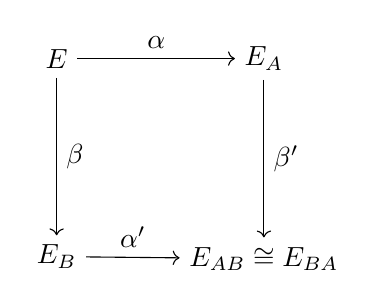
\begin{tikzpicture}[node distance = 2cm]
            \node (E) {$E$};
            \node (EA) [right = of E] {$E_A$};
            \node (EB) [below = of E] {$E_B$};
            \node (EAB) [below = of EA] {$E_{AB} \cong E_{BA}$};
            \draw [->] (E) -- node [above, midway] {$\alpha$} (EA);
            \draw [->] (E) -- node [right, midway] {$\beta$} (EB);
            \draw [->] (EA) -- node [right, midway] {$\beta'$} (EAB);
            \draw [->] (EB) -- node [above, midway] {$\alpha'$} (EAB);
        \end{tikzpicture}
    \end{center}
\end{proof}

\printbibliography

\end{document}